
\chapter{Espaces euclidiens}
\section{Introduction}
Les espaces vectoriels considérés dans ce chapitre sont réels. On suppose que $E$ est un $\R$-espace vectoriel.

Produit scalaire:
\begin{definition}
    Une forme bilinéaire sur $E$ est une application  
    \begin{align*}
        B: E \times E &\longrightarrow \R \\
        (u, v) &\longmapsto B((u, v))
    \end{align*}
    qui vérifie les conditions suivantes $\forall u, v, w \in E$ $\forall \lambda \in \R$:
    \begin{enumerate}
        \item $B(u + \lambda v, w) = B(u, w) + \lambda B(v, w)$
        \item  $B(u, v + \lambda w) = B(u, v) + \lambda B(v, w)$
    \end{enumerate}
    B est dite 
    \begin{enumerate}
        \item symétrique si $B(u, v) = B(v, u)$  $\forall u, v \in E$
        \item positive si $B(., u) \ge 0 \, \forall u \in E$
        \item définie si $B(u, u) = 0 \iff u = 0$
    \end{enumerate}
\end{definition}
\begin{notation}
   Produit scalaire est noté: $<u, v>$ 
\end{notation}
\begin{eg}.
   \begin{enumerate}
       \item $E = \R^n$,  $X = (x_1, \ldots, x_n), Y = (y_1, \ldots, y_n) \in E$\\
           \[
               <X, Y> := \sum_{n=1}^{n} x_iy_i
           \] 
           On l'appelle "produit scalaire canonique"(ou usuel)
        \item $E = \R^2$ et  $<X, Y> = 2x_1y_1 + x_2y_2$
        \item $E = \mathcal{C}^0([-1, 1], \R) \ni f, g$ (un espace des fonctions continues)
            \[
                <f, g> := \int_{-1}^{1} f(t) \cdot g(t) \: d{t} 
            \] 
        \item $E = \mathcal{M}_n(\R) \ni A, B$
             \[
            <A, B> := Tr(A^tB)
            \] 
   \end{enumerate} 
\end{eg}

\begin{prop}
    Un espace vectoriel non-nul possede une infinité de produits scalaires differents.   
\end{prop} 

\begin{definition}
    Un espace euclidien est un couple $(E, < . >)$ où $E$ est un  $\R$-espace vectoriel \underline{de dimension finie} et  $< . >$ est un produit scalaire sur  $E$.
\end{definition}
\begin{property} Soit $(E, < . >)$ un espace euclidien. On pose:
    \[
    \|X\| := \sqrt{<X,X>} \qquad X \in E 
    \] 
    la norme (ou longeur) de $X$. (Il est bien définie car $<., .>$ est toujours positif)
\end{property}
\begin{property}
   Soient $X, Y \in E$, alors:
   \[
       \|X + Y\|^2 = \|X\|^2 + 2\scalair{X, Y} + \|Y\|^2
   \] 
\end{property}
\begin{proof}
   \begin{align*}
       \|X + Y\|^2 = \sqrt{\scalair{X + Y, X + Y}}^2 &= \scalair{X + Y, X + Y} \\ 
                                                     &= \scalair{X, X + Y} + \scalair{Y, X + Y}  \\
                                                     &= \scalair{X, X} + \scalair{X, Y} + \scalair{Y, X} + \scalair{Y, Y}\\
                                                     &= \|X\|^2 + 2\scalair{X, Y} + \|Y\|
   \end{align*} 
\end{proof}
\begin{lemma}\label{lemma:inegalite-cauchy-schwarz} inégalité de Cauchy-Schwarz
   On a
   \[
   |<u, v>| \le \|u\| \cdot \|v\| \qquad \forall u, v \in E
   \] 
   avec égalité si et seulement si $u$ et  $v$ sont colinéaires, i.e  $\exists \, t \in R$ tel que $u = tv$ ou  $v = tu$
\end{lemma}
\begin{explanation}
   Si $v = 0$, clair\\
   Si $v \neq 0$ on considère $\forall t \in \R$
   \begin{align*}
       \|u + tv\|^2 &= <u + tv, u + tv>\\ 
                    &= <u, u + tv> + t<v, u + tv>\\
                    &= <u, u> + t<u, v> + t<v, u> + t^2<v, v>\\
                    &= \|u\|^2 + 2t<u, v> + t^2 \|v\|^2 = f(t)
   \end{align*}
   \begin{center}
       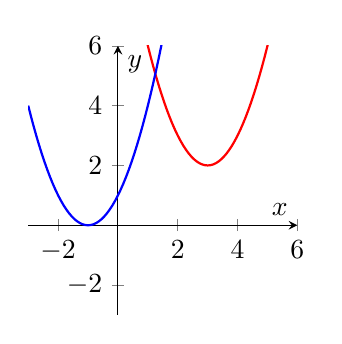
\begin{tikzpicture}
           \begin{axis}[
               axis lines = center,
               xlabel = $x$,
               ylabel = $y$,
               samples = 100,
               domain = -3:6,
               xmin = -3, xmax = 6,
               ymin = -3, ymax = 6,
               width=5cm,
               height=5cm
               ]
               \addplot[red, thick] {(x - 3)^2 + 2};
               \addplot[blue, thick] {(x + 1)^2};
           \end{axis}
       \end{tikzpicture}
   \end{center}
Cas 1: $f(t)$ n'a pas de racinces différentes
\begin{align*}
    &\Delta = 4<u, v>^2 = 4\|u\|^2\|v\|^2 \le 0\\
    \implies & <u, v>^2 \le \|u\|^2 \cdot \|v\|^2\\
    \implies & |<u, v>| \le \|u\|\|v\|
\end{align*}
Cas 2: $f(t)$ a seulement une racine:\\
\begin{align*}
    &\Delta = 0\\
    \implies & \exists t \in \R \text{ tq } \|u + tv\|^2 = 0\\
    \implies &u + tv = 0 \implies u = -tv
\end{align*}
\end{explanation}
La définition suivante sera étudiée dans le cours d'analyse:
\begin{definition}
    On dit que $N: E \to \R_+$ est une norme si:
    \begin{enumerate}
        \item $N(\lambda u) = |\lambda| \cdot N(u)$ \quad  $\forall \lambda \in \R, \forall u \in E$
        \item $N(u) = 0 \implies u = 0$
        \item $N(u + v) \le N(u) + N(v)$ \quad $\forall u, v \in E$
    \end{enumerate}
\end{definition}
\begin{lemma}
   L'application
   \[
   \sqrt{<.,.>} = \| . \|: E \to \R_+ 
   \] 
   est dite norme euclidienne.
\end{lemma}
\begin{explanation}
    1), 2) sont faites\\
    \begin{itemize}
        \item[3)] $\| u + v \|^2 = \|u\|^2 + 2<u,v> + \|v\|^2 \le \|u\|^2 + 2\|u\|\|v\| + \|v\|^2 = (\|u\| + \|v\|)^2$
            \[
            \implies \|u + v\|^2 \le \|u\|^2 + \|v\|^2
            \] 
    \end{itemize}
\end{explanation}
\begin{prop}
   On a les identités suivantes $\forall u, v \in E$ 
   \begin{enumerate}
       \item Identité du parallèlograme:
           \[
           \|u + v\|^2 + \|u - v\|^2 = 2(\|u^2\| + \|v\|^2)
           \] 
       \item Identité de polarisation:
           \[
               \scalair{u, v} = \frac{1}{4}(\|u + v\|^2 - \|u - v\|^2)
           \] 
   \end{enumerate}
\end{prop}
\begin{explanation}.
   \begin{enumerate}
       \item 
           \begin{align*}
               \|u + v\|^2 &= \scalair{u + v, u + v}\\
                           &= \|u\|^2 + 2\scalair{u,v} + \|v\|^2
           \end{align*}
       \item $\|u - v\|^2 = \|u\|^2 - 2\scalair{u, v} + \|v\|^2$
   \end{enumerate} 
   On a:
   \begin{itemize}
       \item 
           $(1) + (2)$:  $\|u + v\|^2 + \|u - v\|^2 = 2 (\|u\|^2 + \|v\|^2)$
       \item $(1) - (2)$:  $\|u + v\|^2 - \|u - v\|^2 = 4\scalair{u, v}$ 
   \end{itemize}
\end{explanation}
\section{Orthogonalité}
Soit $E$ un  $\R$-espace vectoriel et  $\scalair{ , }$ un produit scalaire sur  $E$.
\begin{definition}\label{def:orthogonal}
     $u, v \in E$ sont dits \underline{orthogonaux} si  $<u, v> = 0$. On note  $u \perp v$
      \begin{itemize}
         \item Deux sous-ensembles $A, B$ de  $E$ sont orthogonaux si:
              \[
             \forall u \in A, \forall v \in B, \quad <u, v> = 0
             \] 
         \item Si $A \subseteq E$ on appelle \textbf{orthogonal de $A$}, noté  $A^{\perp}$ l'ensemble
              \[
                  A^{\perp} = \{ u \in E \mid <u, v> = 0 \quad \forall v \in A \}
             \] 
             Aussi connu comme \textbf{orthogonal complement of $A$}
         \item Une famille $(v_1, \ldots, v_n)$ de vecteurs de $E$ est dite orthogonale si  $\forall i \neq j, v_i \perp v_j$. Elle est dite orthonomée si elle est orthogonale et de plus $\|v_i\| = 1 \quad \forall i \in \{ 1, \ldots, n \}$
     \end{itemize}
\end{definition}
\begin{eg}
   $E = \R^n$,  $< , >$ produit scalaire canonique 
   \[
       v_i = (0, \ldots, 0, \underbrace{1}_{i}, 0, \ldots, 0)
   \] 
   \[
   <v_i, v_j> = \begin{cases}
       1 \text{ si } i = j\\  
       0 \text{ si } i \neq  j
   \end{cases}
   \] 
   $(v_1, \ldots, v_n)$ est une base canonique
\end{eg}
\begin{prop}
    \begin{enumerate}
        \item 
            Si $A \subseteq E$ alors $A^{\perp}$ est un sous-espace vectoriel de  $E$ 
        \item Si $A \subseteq B$ alors $B^{\perp} \subseteq A^{\perp}$
        \item $A^{\perp} = Vect(A)^{\perp}$
        \item $A \subset (A^{\perp})^{\perp}$ 
    \end{enumerate}
\end{prop}
\begin{explanation}
   Exercice 
\end{explanation}
\begin{eg}
   \begin{enumerate}
       \item $E = \mathcal{C}^0([-1, 1], \R)$
            \[
                <f, g> := \int_{-1}^{1} f(t) \cdot g(t) \: d{t} 
            \] 
            \begin{center}
       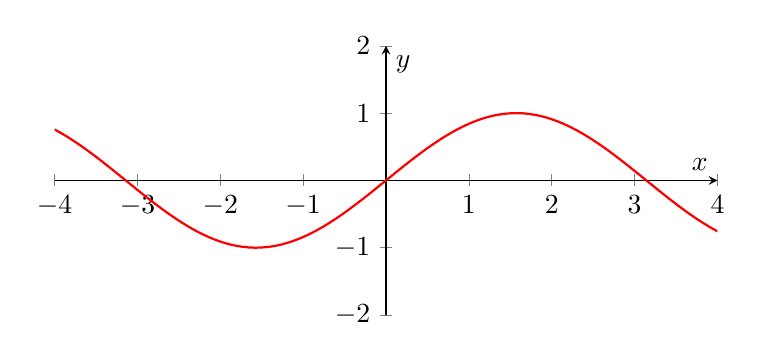
\begin{tikzpicture}
           \begin{axis}[
               axis lines = center,
               xlabel = $x$,
               ylabel = $y$,
               samples = 100,
               domain = -4:4,
               xmin = -4, xmax = 4,
               ymin = -2, ymax = 2,
               width=10cm,
               height=5cm
               ]
               \addplot[red, thick] {sin(deg(x))};
           \end{axis}
       \end{tikzpicture}
   \end{center}
   Alors, $f(t) = \cos(t)$, $g(t) = \sin(t)$ sont orthogonaux: $2\cos(t)\sin(t) = \sin(2t)$
   \[
       \int_{-1}^{1} \cos(t)\sin(t)\:d{t} = \frac{1}{2}\int_{-1}^{1} \sin(2t) \: d{t} = 0  
   \] 
   \end{enumerate} 
\end{eg}
\begin{definition}
    Si $E$ est un espace euclidien, on appelle "dual de $E$" l'ensemble
    \[
        L(E, \R) = \{ f: E \to \R \mid f \text{ est linéaire}\}
    \] 
    On le note $E^*$. Un élément  $f \in E^*$ s'appelle une forme linéaire.
\end{definition}
Rappele:
\begin{prop}
    Si $F, F'$ sont deux e.v de dimension finie, on  $dim(L(F, F')) = dim(F)\cdot dim(F')$\\
    En particulier,  $dim(F^*) = dim(F)$. En effet si  $n = (e_1, \ldots, e_p)$ est une base de $F$ est  $n' = (e'_1, \ldots, e'_q)$ est une base de $F'$, alors l'application
    \begin{align*}
        : L(F, F') &\longrightarrow Mat_{f\times p}(\R) \\
        f &\longmapsto (f) = Mat_{n,n'}(f)
    .\end{align*}
    est un isomorphisme. Donc $dim(F, F) = qp$
\end{prop}
\begin{theorem}
    Théorème du rang: Si  $F$ est un e.v de dimension finie et  $f: F \to F'$ linéaire, alors $dim(F) = dim(Ker(f)) + dim(Im(f))$
\end{theorem}
\begin{prop}
    Si $F, F'$ sont deux e.v \underline{de dimension finie} tq $dim(F) = dim(F')$ et  $f: F \to F'$ linéaire, alors $f$ est un isomorphisme $\iff Ker(f) = {0}$
\end{prop}
\begin{explanation}
   On rappelle que si $G, G'$ sont des sous-e.v de dimension finie dans le même e.v, alors:
   \[
   G = G' \iff G \subseteq G' \text{ et } dim(G) = dim(G')
   \] 
   $\implies$) $f$ injective  $\implies$ $Ker(f) = {0}$\\
   $\impliedby$) Soit $Ker(f) = {0}$.\\
   Alors, forcément  $dim(Ker(f)) = 0$ et par le théorème du rang on a  $dim(F) = dim(Im(f))$, donc  $Im(f) = F'$
\end{explanation}
\begin{lemma} du Riesz:\\
    Soit $(E, \scalair{.,.})$ un espace euclidien de  dimension finie et $f \in E^*$. Alors, $\exists! u \in E$ tel que $f(x) = \scalair{u, x} \quad \forall x \in E$. La forme linéaire $f$ est donné par un produit scalaire avec un vecteur. 
\end{lemma}
\begin{notation}
   Pour tout $v \in E$ on note par  $f_v$ l'application:
   \begin{align*}
       f_v: E &\longrightarrow \R \\
       x &\longmapsto f_v(x) = <v, x>
   .\end{align*}
   $f_v$ est linéaire  $\forall v \in E$ i.e $E^*$
\end{notation}
\begin{explanation} lemma de Reisz\\
   On considère l'application
   \begin{align*}
       \phi: E &\longrightarrow E^* \\
       v &\longmapsto \phi(v) = f_v
   .\end{align*}
   $\phi$ est linéaire (exercice).  $\phi$ est injective:
   \[
   v \in Ker(\phi) \iff f_v(x) = 0 \quad \forall x \in E
   \] 
   en particulier pour x = v, on a:
   \[
   0 = f_v(v) = <v,v> \implies v = 0
   \] 
   \begin{align*}
       dim(E) = dim(E^*) &\implies \phi \text{ est un isomorphisme}\\
                         &\implies \phi \text{ bijective}
   \end{align*}
   \[
   \forall f \in E^*, \exists! n \in E \text{ tq } \phi(n) = f, \text{ i.e } f(x) = <n, x> \, \forall x \in E
   \] 
   Dans ce cas $E = \R^n$, le lemme de Riesz est tres simple à comprendre:\\
   Soit  $f: \R^n \to \R$ une forme linéaire. Si on note $(e_1, \ldots, e_n)$ la base canonique de $\R^n$, tout $x \in \R^n$ s'écrit 
    \begin{align*}
        x = \sum_{n=1}^{n} \alpha_ie_i \qquad \alpha_i \in \R, \forall i \in \{1, \ldots, n\}\\
        \implies f(x) = \sum_{n=1}^{n} \alpha_if(e_i) = <(\alpha_1, \ldots, \alpha_n), (a_1, \ldots, a_n)> = <(a_1, \ldots, a_n), (\alpha_1, \ldots, \alpha_n)>
   \end{align*}
\end{explanation}
